\section{Архитектура распределённой системы}

Высокоуровневая архитектура системы основана на разделении функций координации
и непосредственного выполнения вычислений. В системе выделяются три основных
компонента: клиент, кластер узлов консенсуса Raft и набор вычислительных узлов
(рабочий). Такое разделение соответствует классической модели разделения
\emph{control plane} и \emph{data plane}: кластер Raft отвечает за
согласование, хранение и изменение глобального состояния, а рабочие узлы
исполняют пользовательские задачи, не принимая решений, влияющих на
консистентность всей системы \cite{coulouris2012}. Общая схема взаимодействия
показана на рис.~\ref{fig:arch-overview}.

\begin{figure}[h]
    \centering
    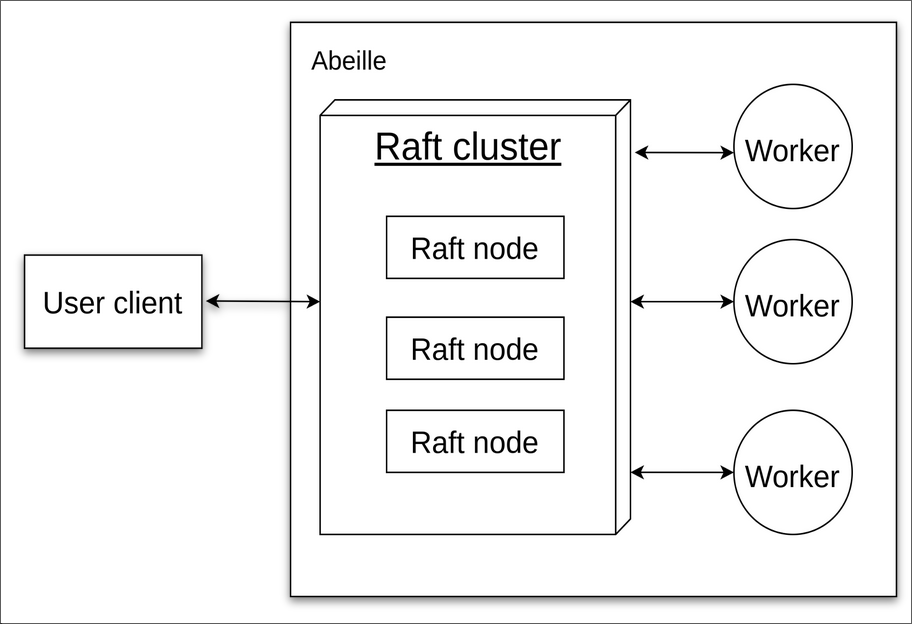
\includegraphics[width=0.82\linewidth]{inc/arch-overview.png}
    \caption{Высокоуровневая архитектура распределённой системы}
    \label{fig:arch-overview}
\end{figure}

Клиент взаимодействует только с кластером Raft. Это означает, что любая
операция, изменяющая состояние системы, сначала попадает на один из узлов
кластера, при необходимости перенаправляется лидеру, затем записывается в лог
Raft, реплицируется на большинство узлов и только после этого считается
подтверждённой. Такой подход позволяет использовать кластер как единственный
источник истины о состоянии распределённой системы. В частности, через него
фиксируются постановка задач, назначение задачи конкретному рабочему узлу,
изменение статуса выполнения и сохранение итогового результата. Благодаря этому
система получает детерминированный порядок событий и устойчивость к повторам
запросов, сетевым задержкам и частичным отказам.

Кластер Raft играет роль координационного центра. Его узлы поддерживают
реплицированную машину состояний, принимают клиентские запросы, выполняют их
валидацию и принимают решения о диспетчеризации задач. После коммита новой
операции в машине состояний лидер может безопасно передать задание
вычислительному узлу. Аналогично и обратный поток данных организован через
кластер: рабочий не отправляет результат напрямую клиенту, а возвращает его в
кластер, где он также проходит через запись в лог и коммит. Лишь после этого
результат становится наблюдаемым для клиента. Таким образом, даже при отказе
отдельного узла или смене лидера система сохраняет согласованность состояния и
не допускает появления «локально известных», но глобально не подтверждённых
результатов.

Вычислительные узлы образуют исполнительный контур системы. Их задача состоит в
получении заданий от кластера, выполнении пользовательского кода и передаче
результатов обратно. В предлагаемой архитектуре рабочие узлы остаются
максимально простыми: они не участвуют в алгоритме консенсуса, не
координируются между собой и не принимают решений о глобальном состоянии
системы. Это делает их удобными для масштабирования: увеличение числа рабочих
повышает вычислительную пропускную способность системы без усложнения протокола
согласования. Иными словами, консенсусный контур остаётся компактным и
управляемым, а исполнительный контур --- эластичным.

Принципиальным архитектурным решением является отказ от прямого взаимодействия
между клиентом и рабочими узлами, а также отказ от горизонтального взаимодействия
между самими рабочими узлами. Такое ограничение уменьшает связанность системы и
упрощает обеспечение корректности. Во-первых, все проверки аутентификации,
авторизации, квот и политик исполнения могут быть сосредоточены в одном месте
--- в кластере Raft. Во-вторых, единая точка сериализации операций устраняет
риск расхождения состояния при сетевых разделениях и гонках между несколькими
исполнителями. В-третьих, вычислительные узлы можно проектировать как
практически без состояния или со слабо связанным локальным состоянием, что
существенно упрощает их замену, перезапуск и масштабирование.

С точки зрения отказоустойчивости система ориентирована на модель
crash-stop/crash-recovery и частично синхронную сеть. Безопасность кластера
обеспечивается алгоритмом Raft: два различных значения не могут быть
закоммичены в одной и той же позиции лога, а после выбора нового лидера
система продолжает работу с согласованного состояния \cite{ongario2014}. При
отказе отдельного рабочего узла целостность системы не нарушается, поскольку
состояние задачи уже зафиксировано в машине состояний и может быть использовано
для повторного назначения. При отказе лидера выполняется переизбрание, и после
достижения кворума обслуживание запросов продолжается. Для кластера из $N$
узлов консенсуса система сохраняет работоспособность при отказе до
$\lfloor (N-1)/2 \rfloor$ узлов, что соответствует стандартной кворумной
гарантии \cite{lynch1996}.

Рассматривались и альтернативные варианты построения системы: прямой доступ
клиента к рабочим узлам, объединение ролей вычислительных и консенсусных узлов,
а также более децентрализованные схемы взаимодействия исполнителей. Однако
такие решения либо увеличивают поверхность ошибок и сложность сопровождения,
либо ухудшают масштабируемость за счёт роста числа участников консенсуса.
Выбранная архитектура, напротив, позволяет чётко локализовать инварианты
безопасности внутри кластера Raft и одновременно сохранить простоту
вычислительного контура. Поэтому она является наиболее подходящей для системы
распределённых вычислений, в которой критически важны согласованность,
отказоустойчивость и предсказуемое масштабирование.
